%% India HCI 2026 submission — single-column ACM review format.
%% Compile on Overleaf or any TeX Live install with the acmart class.
%% Switch to \documentclass[sigconf]{acmart} for the 2-column camera-ready.
\documentclass[manuscript,review,anonymous]{acmart}

\AtBeginDocument{%
  \providecommand\BibTeX{{%
    Bib\TeX}}}

%% Rights/metadata are placeholders for the anonymous review build.
\setcopyright{acmlicensed}
\copyrightyear{2026}
\acmYear{2026}
\acmDOI{XXXXXXX.XXXXXXX}
\acmConference[India HCI '26]{Proceedings of the 16th Indian Conference on Human-Computer Interaction}{October 29--31, 2026}{India}
\acmISBN{978-1-4503-XXXX-X/2026/10}

\begin{document}

\title{The Flow Dial: A Selection-Free Circular Keyboard for Noisy Cursor-Driven Brain--Computer Interfaces}

%% Anonymous review build: acmart hides author identity automatically.
\author{Anonymous Author(s)}
\affiliation{%
  \institution{Submission to India HCI 2026}
  \country{}}

\renewcommand{\shortauthors}{Anonymous}

\begin{abstract}
Intracortical brain--computer interfaces (BCIs) such as Neuralink let people
move an on-screen cursor by attempted or imagined movement, but text entry
remains a bottleneck. Most on-screen keyboards for such cursors are built around
\emph{target acquisition followed by selection} (dwelling or clicking) --- yet
holding a noisy, fatigue-prone cursor still on a small key, and producing a
discrete ``click'', are precisely the two operations a brain-driven cursor
performs worst. We present the \emph{Flow Dial}, a circular text-entry method
that is \emph{continuous and selection-free}: candidate characters occupy
angular arcs around a central rest zone, the angular width of each arc grows
with the language-model probability of that character, and a character is
committed simply by flowing outward through its arc until the cursor crosses an
outer ring. There is no dwell and no click. Because we cannot ethically or
practically run an implanted-BCI study at this stage, we evaluate the
\emph{mechanic} with a noisy-cursor simulation that drives the Flow Dial and a
conventional point-and-dwell baseline through the same cursor model, sweeping a
motor-noise parameter that stands in for degrading signal quality. The Flow Dial
degrades gracefully (from $\approx$37 to $\approx$24 effective words per minute
as noise grows) while the dwell baseline collapses below 1 wpm and its error
rate exceeds 70\%. An ablation that removes the language model confirms that the
predictive arc-sizing is essential under noise --- which also predicts the
design's honest limitation on low-redundancy input such as source code. We
release an open, mouse-drivable prototype with a built-in study mode that logs
standard text-entry metrics, so the simulation can be complemented by a
surrogate-cursor human study. We frame the contribution as a design and a
reproducible, hardware-free evaluation methodology rather than an
implant-validated performance claim.
\end{abstract}

\begin{CCSXML}
<ccs2012>
 <concept>
  <concept_id>10003120.10003121.10003122.10003334</concept_id>
  <concept_desc>Human-centered computing~Text input</concept_desc>
  <concept_significance>500</concept_significance>
 </concept>
 <concept>
  <concept_id>10003120.10003121.10003124.10010870</concept_id>
  <concept_desc>Human-centered computing~Interaction techniques</concept_desc>
  <concept_significance>500</concept_significance>
 </concept>
 <concept>
  <concept_id>10003120.10003138.10003141</concept_id>
  <concept_desc>Human-centered computing~Accessibility technologies</concept_desc>
  <concept_significance>300</concept_significance>
 </concept>
</ccs2012>
\end{CCSXML}

\ccsdesc[500]{Human-centered computing~Text input}
\ccsdesc[500]{Human-centered computing~Interaction techniques}
\ccsdesc[300]{Human-centered computing~Accessibility technologies}

\keywords{text entry, brain--computer interface, cursor control, circular
keyboard, continuous input, language models, accessibility, simulation}

\maketitle

\section{Introduction}
Recent intracortical brain--computer interfaces (BCIs), including the publicly
demonstrated Neuralink system, restore digital autonomy by letting a person move
a cursor on a screen through attempted or imagined movement. The headline metric
for such systems is pointing throughput, often reported in bits per second on a
target-acquisition task. Text entry, however, lags well behind pointing: it
inherits all of the difficulty of controlling a noisy cursor and then adds the
requirement of selecting one small symbol after another.

Two properties of a brain-driven cursor matter for keyboard design. First, the
cursor is a \emph{noisy two-dimensional point}: the decoded velocity or position
estimate jitters, so small, tightly packed targets are hard to hit and hard to
hold. Second, the costly, fatiguing operations are \emph{holding the cursor
still} on a target and producing a discrete \emph{selection} (a dwell or an
attempted click). Most existing on-screen keyboards for gaze and BCI control are
nonetheless built around exactly these operations: the user acquires a key and
then dwells on it or clicks to select. The interaction asks the device to do the
two things it is worst at, once per character.

We take the opposite stance. We ask: what is the least effortful thing a
brain-driven cursor can reliably do, and how can text be produced from
\emph{that}? Steering a heading --- leaning the cursor in a direction and letting
it travel --- is comparatively easy and does not require stopping. Building on
this observation, and on a lineage of continuous, language-model-driven text
entry, we present the \emph{Flow Dial}: a circular keyboard in which the user
never stops and never clicks.

In the Flow Dial, the screen is a disc with a small central rest zone. Candidate
characters occupy angular arcs around the disc. The angular width of each arc is
proportional to the probability that its character comes next, given the
previously entered character, under a language model. The user enters a
character by flowing the cursor outward, in the direction of the desired arc,
until it crosses an outer commit ring; whichever arc the heading lies in at the
crossing is committed. The cursor then drifts back through the centre, where the
next set of likely characters has already grown large. There is no dwell timer
and no selection gesture.

This design produces three properties we believe are well matched to a noisy
cursor. (1)~Returning to a neutral, central rest position is essentially free,
rather than being another deliberate acquisition. (2)~The characters most likely
to be needed next are the largest and easiest to hit, so common cases tolerate
sloppy control. (3)~Selection is folded into motion, removing the dwell/click
operation entirely.

We cannot, at this stage, evaluate the Flow Dial on an implanted device; doing so
would require clinical access and ethical approval far beyond the scope of an
initial design contribution. We therefore make a deliberately scoped,
\emph{relative} claim and test it with a reproducible simulation. We model the
cursor as a point driven toward an on-screen goal by a proportional controller
with additive Gaussian motor noise, and we drive both the Flow Dial and a
conventional point-and-dwell keyboard with the \emph{same} cursor. By sweeping
the motor-noise level --- our stand-in for degrading BCI signal quality --- we
compare how the two \emph{mechanics} behave as the cursor worsens. We also ablate
the language model to separate the contribution of the geometry from that of
prediction.

This paper makes the following contributions:
\begin{itemize}
\item \textbf{The Flow Dial}, a selection-free circular text-entry method for
  noisy cursor-driven BCIs, in which language-model probability is mapped to the
  angular width of continuous commit arcs.
\item \textbf{A hardware-free evaluation methodology}: a shared noisy-cursor
  simulation that compares the Flow Dial against a point-and-dwell baseline as a
  function of cursor noise, plus a language-model ablation.
\item \textbf{Empirical (simulated) evidence} that the Flow Dial degrades
  gracefully under noise where the baseline collapses, and that the language
  model is essential to this robustness --- which in turn predicts an honest
  limitation on low-redundancy input such as code.
\item \textbf{An open, mouse-drivable prototype} with a built-in study mode that
  logs standard text-entry metrics, enabling a surrogate-cursor human study as a
  direct follow-up.
\end{itemize}

We are explicit about what we do \emph{not} claim: we do not report
implant-validated entry rates, and our absolute numbers depend on parameters of
the cursor model that we state openly and treat as assumptions.

\section{Related Work}
\subsection{Text entry for BCIs and gaze}
Intracortical BCIs have advanced rapidly from cursor control to higher-bandwidth
communication. Approaches to BCI text entry include point-and-select spellers,
imagined-handwriting decoding, and decoding of attempted speech or finger
movements. These differ in the signal they decode, but a cursor-control BCI in
particular presents text entry as a pointing problem, where speed is bounded by
the throughput and stability of the decoded cursor rather than by the user's
intent to type a particular letter. Gaze-based communication faces a structurally
similar challenge, and gaze typing by dwell is well known to be slow and
fatiguing, which has motivated continuous alternatives.

\subsection{Continuous, language-model-driven entry}
Dasher is the canonical continuous-pointing text entry interface: letters are
arranged so the user writes by steering through a zooming world of characters
whose sizes are set by a language model, never stopping to select. Dasher
reaches roughly 25 words per minute by mouse and substantially outperforms dwell
based eye-typing when driven by gaze, and speech-augmented variants go faster
still. The Flow Dial shares Dasher's core commitments --- continuous control and
probability-driven target sizing --- but reorganises them into a fixed radial
layout with a free central rest position and an explicit outward ``flow to
commit'' action, which we hypothesise suits a cursor whose easiest control
dimension is heading and whose neutral position should be cost-free.

\subsection{Circular and radial keyboards}
Radial and pie-menu layouts have a long history in HCI and have been applied to
text entry on smartwatches, in virtual reality, and for gaze. Circular gaze
keyboards that arrange letters by frequency with word prediction are deployed in
assistive contexts. A recurring finding is that unfamiliar radial layouts impose
a learning cost relative to QWERTY, and that word/character prediction
substantially boosts throughput. Word-gesture (shape-writing) keyboards likewise
show that continuous strokes plus a language model can be both fast and
error-tolerant. The Flow Dial differs from frequency-ordered circular keyboards
in that it is selection-free: characters are not dwelled upon or tapped but
committed by crossing a ring, and arc \emph{width} (not just position) encodes
prediction.

\subsection{Modelling and simulation for keyboard design}
Comparing keyboard layouts and mechanics through models --- Fitts' law movement
time weighted by corpus statistics, and Monte-Carlo simulation of noisy
selection --- is a long-standing and accepted practice that complements, and
often precedes, human trials. Surrogate-input or input-emulation studies (driving
an interface with a deliberately degraded mouse, a trackpad, or an eye-tracker)
are similarly used when the target device is unavailable. We adopt both: a
noisy-cursor simulation for the central comparison, and an instrumented prototype
to enable a surrogate-cursor pilot.

\section{The Flow Dial}
\subsection{Layout and rest zone}
The Flow Dial occupies a circular region. At its centre is a small
\emph{rest zone}; while the cursor is inside it, no commit can occur and the
dial is ``armed''. Around the disc, the full character set (here, 26 letters
plus space, with backspace as an additional arc) is laid out as a set of angular
\emph{arcs} that together tile the full circle. Two concentric radii matter: the
rest-zone radius, and an outer \emph{commit ring}.

\subsection{Prediction-driven arc width}
Let $c_{\text{prev}}$ be the most recently committed character and let
$P(c \mid c_{\text{prev}})$ be a language model's probability that character $c$
comes next. The Flow Dial sets the angular width $w(c)$ of each arc proportional
to a compressed function of this probability,
\[
  w(c) \;\propto\; \sqrt{P(c \mid c_{\text{prev}})},
\]
normalised so the arcs fill $2\pi$. The square root compresses the dynamic range
so that very likely characters get wide, easy arcs while rare characters remain
reachable rather than vanishing; a probability floor (from add-$k$ smoothing in
the model) guarantees every character always has a non-zero arc. Because the
layout re-sizes after every commit, the characters most likely to be needed next
are always the largest targets.

\subsection{Flow-to-commit}
To enter a character, the user moves the cursor outward from the rest zone in
the direction of the desired arc. When the cursor crosses the commit ring, the
arc that contains the cursor's current heading is committed. The cursor then
returns through the centre; re-entering the rest zone re-arms the dial
(a hysteresis that prevents a single outward motion from committing twice). No
dwell time elapses and no click is issued: \emph{selection is a side effect of
motion}. Backspace is itself an arc, so corrections use the same gesture.

\subsection{Why this should suit a noisy cursor}
The design embodies three principles drawn from the device's characteristics.
\emph{Free rest:} returning to neutral is automatic, not a separate acquisition,
which we expect reduces sustained effort. \emph{Forgiving common case:} the
high-probability characters occupy wide arcs, so the cursor can be imprecise and
still land correctly most of the time. \emph{No stop, no click:} the two
operations a brain-driven cursor performs worst are removed. The cost we accept
in exchange is a dependence on next-character predictability, which we examine
directly in our ablation.

\section{Evaluation Method}
\subsection{Rationale and scope}
We evaluate the Flow Dial \emph{mechanic} rather than an implanted system. The
question we answer is relative and mechanistic: as a single cursor becomes
noisier, how do a selection-free flow mechanic and a conventional point-and-dwell
mechanic compare in speed and accuracy, and how much of any difference depends on
the language model? We hold the cursor model identical across mechanics so that
differences are attributable to the interaction technique, not to the input
device. We explicitly do not claim implant-validated words-per-minute.

\subsection{Shared noisy-cursor model}
Both mechanics are driven by the same cursor. At each timestep of duration
$\Delta t$, the cursor position is updated by a proportional controller toward an
on-screen goal, plus additive Gaussian motor noise:
\[
  \mathbf{p}_{t+1} \;=\; \mathbf{p}_t \;+\; g\,(\mathbf{goal}-\mathbf{p}_t)\,\Delta t \;+\; \boldsymbol{\eta}, \qquad \boldsymbol{\eta}\sim\mathcal{N}(0,\sigma^2 I).
\]
The noise standard deviation $\sigma$ is the single swept parameter; it stands in
for worsening BCI signal quality. The gain $g$ and timestep $\Delta t$ are held
fixed and reported as assumptions. For the Flow Dial, the goal is a point just
beyond the commit ring along the intended arc's midline, and the committed
character is whichever arc contains the heading at ring crossing; a return trip to
the centre is simulated (and charged) between characters. For the baseline, the
goal is the intended fixed key, and selection requires the cursor to remain
within a key's hit region for a fixed dwell; if the cursor dwells in a
neighbouring key, that is a mis-selection.

\subsection{Conditions}
We use a $3\times 8$ design. The three techniques are: \textbf{Flow Dial
(+prediction)}, the proposed system with arc widths from a bigram language model;
\textbf{Flow Dial (--prediction)}, an ablation with arc widths set by unigram
frequency only; and \textbf{Point-dwell baseline}, 27 fixed keys on a ring with
hold-to-select. The eight noise levels span a clean cursor to a severely degraded
one ($\sigma$ from $0.02$ to $0.20$ in normalised screen units). Each of the 24
cells is repeated over 12 independent random seeds; we report means with 95\%
confidence intervals (normal approximation).

\subsection{Task, corpus and measures}
The task is to transcribe a set of common English phrases. The language model is
a smoothed bigram model estimated from a compact embedded English corpus, so the
experiment is fully reproducible offline; the model conditions next-character
probability on the previously \emph{intended} character. We report effective
words per minute (5 characters per word, including the time of return trips and
of corrections), and character error rate (the fraction of committed characters
that differ from the intended character). A wrong commit is charged a correction
of comparable effort.

\subsection{Instrumented prototype and pilot protocol}
Alongside the simulation we release a browser-based, mouse-drivable Flow Dial.
It includes a study mode that prompts the same phrases, logs every commit
(intended versus actual character, inter-commit time, correctness), and computes
per-phrase words per minute, character error rate, and keystrokes per character,
exporting a CSV. This enables a surrogate-cursor pilot ($N=3$--$5$ participants
driving the dial with a mouse, trackpad, or eye-tracker, with prediction and a
``tremor'' noise injection as within-subject conditions) and the collection of
subjective workload (e.g., NASA-TLX) as an immediate follow-up.

\section{Results}
\subsection{Speed degrades gracefully}
Table~\ref{tab:wpm} and Figure~\ref{fig:wpm} report effective words per minute as
a function of cursor noise. With a near-clean cursor all three techniques are
broadly comparable (35--40 wpm). As noise increases, the point-dwell baseline
collapses: its dwell repeatedly fails to stabilise on the intended key, and by
$\sigma=0.10$ it has fallen to roughly 3 wpm and by $\sigma=0.16$ below 1 wpm.
The Flow Dial declines gently over the same range, from about 37 to about 27 wpm
with prediction. At $\sigma=0.16$ the Flow Dial with prediction is more than an
order of magnitude faster than the baseline.

\begin{table}[t]
  \caption{Effective words per minute (mean over 12 seeds; $\pm$ values in the
  text are 95\% CIs) at representative cursor-noise levels.}
  \label{tab:wpm}
  \begin{tabular}{lcccc}
    \toprule
    Technique & $\sigma{=}0.04$ & $\sigma{=}0.10$ & $\sigma{=}0.16$ & $\sigma{=}0.20$ \\
    \midrule
    Flow Dial (+pred.) & 36.8 & 31.1 & 26.7 & 24.3 \\
    Flow Dial ($-$pred.) & 35.0 & 27.8 & 24.2 & 22.6 \\
    Point-dwell baseline & 31.4 & 3.0 & 0.9 & 0.9 \\
    \bottomrule
  \end{tabular}
\end{table}

\begin{figure}[t]
  \centering
  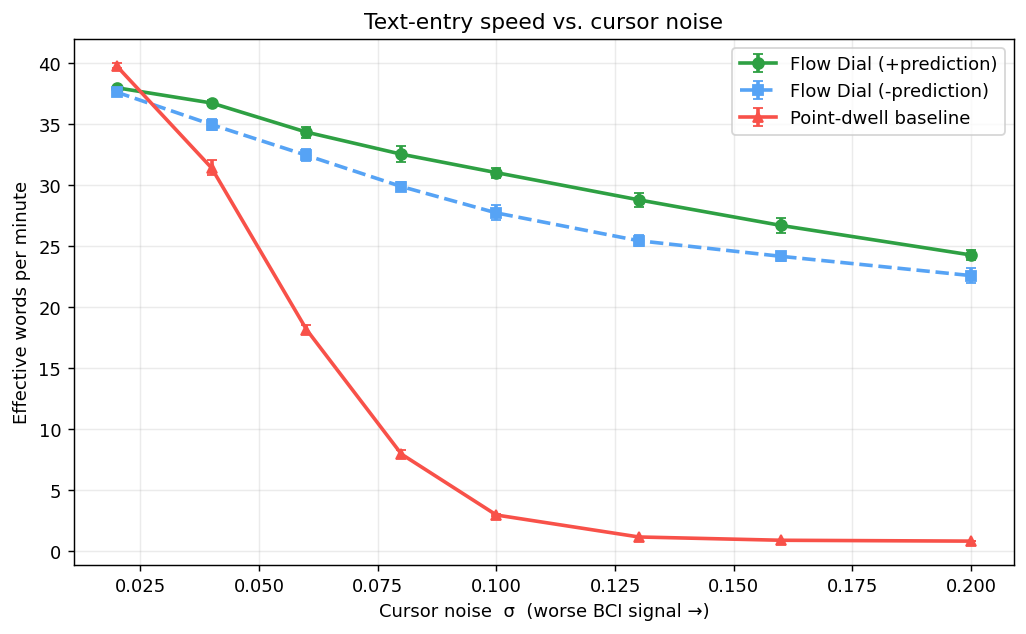
\includegraphics[width=\linewidth]{figures/fig_wpm_vs_noise.png}
  \caption{Effective words per minute versus cursor noise $\sigma$. The
  point-dwell baseline collapses as noise grows, while the Flow Dial (with and
  without prediction) declines gently. Error bars are 95\% confidence intervals
  over 12 seeds.}
  \Description{A line chart with cursor noise sigma on the horizontal axis from
  0.02 to 0.20 and effective words per minute on the vertical axis. Three series
  are shown. The point-dwell baseline starts near 40 words per minute at low
  noise and drops steeply to under 1 word per minute by sigma 0.16. The two Flow
  Dial series start near 37 words per minute and decline gradually to the low 20s
  across the full noise range, with the prediction-enabled series consistently
  above the prediction-disabled series.}
  \label{fig:wpm}
\end{figure}

\subsection{Errors stay bounded}
Table~\ref{tab:cer} and Figure~\ref{fig:err} report character error rate. At every
noise level the Flow Dial with prediction has the lowest error rate. The
baseline's error rises steeply because tremor pushes the cursor into neighbouring
fixed keys, exceeding 70\% at high noise; the Flow Dial with prediction remains
markedly lower across the range.

\begin{table}[t]
  \caption{Character error rate (\%) at representative cursor-noise levels.}
  \label{tab:cer}
  \begin{tabular}{lcccc}
    \toprule
    Technique & $\sigma{=}0.04$ & $\sigma{=}0.10$ & $\sigma{=}0.16$ & $\sigma{=}0.20$ \\
    \midrule
    Flow Dial (+pred.) & 2.1 & 19.5 & 37.5 & 48.0 \\
    Flow Dial ($-$pred.) & 6.4 & 32.6 & 51.2 & 60.6 \\
    Point-dwell baseline & 15.8 & 46.2 & 74.8 & 78.5 \\
    \bottomrule
  \end{tabular}
\end{table}

\begin{figure}[t]
  \centering
  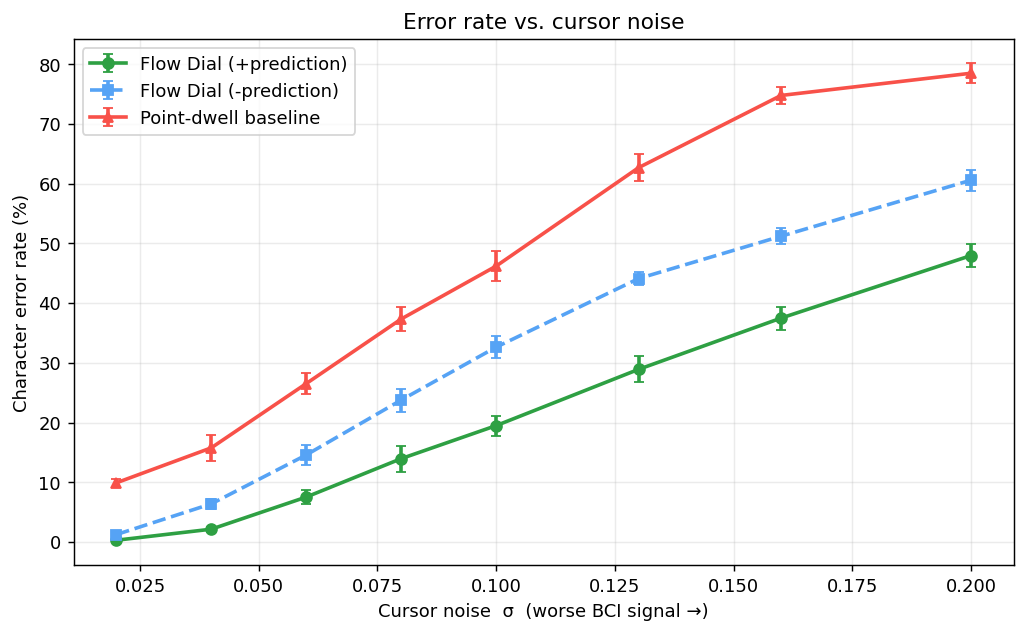
\includegraphics[width=\linewidth]{figures/fig_error_vs_noise.png}
  \caption{Character error rate versus cursor noise $\sigma$. The Flow Dial with
  prediction maintains the lowest error rate at every noise level. Error bars are
  95\% confidence intervals over 12 seeds.}
  \Description{A line chart with cursor noise sigma on the horizontal axis from
  0.02 to 0.20 and character error rate as a percentage on the vertical axis.
  The point-dwell baseline rises fastest, exceeding 70 percent at high noise. The
  Flow Dial without prediction is intermediate, and the Flow Dial with prediction
  has the lowest error rate throughout, rising from about 2 percent at low noise
  to about 48 percent at the highest noise level.}
  \label{fig:err}
\end{figure}

\subsection{Prediction is doing real work}
The +prediction and --prediction curves separate increasingly with noise. At
$\sigma=0.10$, prediction reduces character error rate from about 33\% to about
20\% and raises effective words per minute from about 28 to about 31. This
confirms that the mechanic and the predictive arc-sizing are coupled: the radial
geometry helps on its own, but the language model is what keeps error bounded as
the signal degrades.

\section{Discussion}
\subsection{Why the baseline collapses and the dial does not}
The point-dwell baseline fails under noise for a structural reason: it requires
the cursor to be simultaneously \emph{at} and \emph{still on} a small target, and
both conditions become improbable as $\sigma$ grows, so selections either fail to
register or land on a neighbour. The Flow Dial converts the same noisy motion into
text differently. It only requires that the heading lie within an arc at the
moment of ring crossing, and the arcs that matter most are made wide by
prediction. Noise still causes errors --- the Flow Dial's error rate is not
negligible at high $\sigma$ --- but speed does not collapse, because the
commit does not depend on stillness.

\subsection{An honest limitation: low-redundancy input}
The ablation is not merely a control; it is a forecast. Because the Flow Dial's
robustness leans on next-character predictability, any input whose
next-character distribution is flat will behave like the --prediction condition,
which is consistently worse. Source code is the obvious example: identifiers,
symbols, and mixed-case tokens carry far less of the redundancy that a
natural-language bigram model exploits. We therefore position the Flow Dial as a
strong design for natural-language entry on a noisy cursor and flag structured or
code entry as future work, where a different arc-sizing model or a hybrid with an
explicit symbol layer would be required.

\subsection{Threats to validity}
Our absolute numbers depend on the cursor model. The gain, timestep, dwell time,
key and arc geometry, and the noise range are assumptions; we report them and
treat the comparison as relative. The proportional-controller-plus-Gaussian-noise
model is a simplification of intracortical cursor dynamics, which exhibit
temporally correlated noise and user adaptation that our model omits. The corpus
is small and English-only, and the language model is a bigram model; richer
models would likely help the +prediction condition more than the baseline. Most
importantly, simulation cannot establish learnability, fatigue, or subjective
acceptance. These require human data, which our released prototype is built to
collect; a surrogate-cursor pilot is the natural next step, and an
implanted-device study the eventual one.

\subsection{Design implications}
Two implications generalise beyond the Flow Dial. First, for fatigue- and
noise-limited cursors, making the neutral position \emph{free} --- rather than a
target to be acquired --- may matter as much as layout optimisation. Second,
mapping prediction to \emph{target size} in a continuous, selection-free mechanic
is a robust way to spend a language model's information: it widens the margin for
error exactly where it is needed, instead of merely re-ordering discrete keys.

\section{Conclusion}
We presented the Flow Dial, a selection-free circular keyboard for noisy
cursor-driven BCIs that removes the two operations such cursors perform worst ---
holding still and clicking --- by committing characters through continuous
outward motion and by sizing prediction-driven commit arcs. In a reproducible,
hardware-free simulation that drives both the Flow Dial and a conventional
point-and-dwell keyboard through the same noisy cursor, the Flow Dial degraded
gracefully where the baseline collapsed, and an ablation showed the language
model to be essential to this robustness. We release a mouse-drivable prototype
with built-in metric logging to support a surrogate-cursor human study. We offer
the design and its evaluation methodology as a starting point, and are explicit
that implant-validated performance remains future work.

\section*{Ethics and Privacy Statement}
This work proposes an assistive text-entry method intended to benefit people who
rely on cursor-driven BCIs, a population for whom communication bandwidth
directly affects autonomy. Our evaluation uses simulation and, prospectively, a
surrogate-cursor study with able-bodied volunteers driving a mouse or
eye-tracker; no clinical or neural data are collected, and the released prototype
logs only task performance (typed text and timing) locally, with export under the
participant's control. We caution that the method's reliance on language-model
prediction could, if deployed naively, bias entry toward frequent words or leak
information about likely content; deployments should keep the language model
on-device and give users control over prediction. We make no implant-validated
performance claims, to avoid overstating readiness for clinical use.

%% Acknowledgments omitted in the anonymous review build.

\bibliographystyle{ACM-Reference-Format}
\bibliography{flow_dial}

\end{document}
